% Independent ICASSP 2027 working manuscript. See README.md for evidence status.
\documentclass{article}
\usepackage{spconf,amsmath,amssymb,graphicx,booktabs,hyperref}
\usepackage{tikz}
\usetikzlibrary{arrows.meta,positioning}
\newcommand{\KLA}{\operatorname{KLA}}
\newcommand{\osc}{\operatorname{osc}}
\newcommand{\diag}{\operatorname{diag}}
\title{Delivery-Aware Sparse Causal Routing for Distributed Multi-Object Tracking}
\name{Jinhao Chen \qquad Tianyu Wo\thanks{Corresponding author: Tianyu Wo.}}
\address{Beihang University, Beijing, China}
\begin{document}
\maketitle
\begin{abstract}
We study sparse communication for distributed labeled multi-Bernoulli tracking
when mobile formations change their physical neighbors. A causal routing
policy retains a feasible formation tree, repairs it only when necessary, and
combines local directed cycles with bidirectional gateways. The scheduled
backbone uses $N+2(F-1)$ posterior messages for $N$ sensors in $F$ formations.
We distinguish this planned graph from packet delivery and label-specific
fusion, and derive a finite-round sensitivity bound for exact geometric
fusion. Paired 160-step development experiments with 24 and 36 sensors reduce
attempted posterior bytes by 10.0\% and 21.8\% relative to fixed routing.
Conditional localization RMSE decreases substantially, but set-error gains
are smaller and a consistency tradeoff remains at 36 sensors. These results
motivate delivery-aware receiver weighting while identifying the limits of
connectivity alone as a design objective.
\end{abstract}
\begin{keywords}
Multi-object tracking, labeled multi-Bernoulli, distributed fusion, dynamic
topology, packet loss
\end{keywords}

\section{Introduction}
Mobile sensor formations exchange local posteriors to track objects beyond
individual fields of view. As formations move, an initial route can lose
an inter-formation connection even when an alternative physical link exists.
Retaining many inputs improves redundancy but repeatedly transmits
multi-object densities. The design problem is which posteriors reach which
receivers within a finite tracking interval.

The labeled multi-Bernoulli (LMB) filter represents uncertain object existence
and labeled spatial states \cite{reuter2014lmb}. Consensus LMB filtering uses
Kullback--Leibler averaging (KLA), equivalently normalized geometric fusion,
to combine these densities \cite{battistelli2014kla,fantacci2015consensus}. Its classical
equal-weight consensus limit assumes an appropriate stochastic matrix and
repeated fusion of fixed inputs. A mobile tracker instead alternates local
Bayesian updates with a limited number of communication rounds. A connected
scheduled graph consequently does not establish either successful delivery
or an improvement in tracking error.

Randomized gossip relates averaging time to the spectrum of an appropriate
stochastic matrix \cite{boyd2006gossip}. Event-triggered Bayesian filtering
compares a posterior with its prediction from the last transmission to
trigger communication \cite{battistelli2019event}. Our focus is sparse route
repair under changing physical feasibility and the inputs actually received
for multi-object fusion, rather than a mixing-rate objective or a
posterior-divergence trigger.

Different fields of view introduce another distinction: absence of a label
at one sensor is not always evidence that the object has disappeared.
Multi-view GCI methods address this mismatch at the density-fusion level
\cite{li2019multiview}. Our focus is the communication structure and its
receiver-side realization. The topology comparison keeps the underlying
mixture-aware fusion approximation fixed. The routing policy uses physical
link information rather than posterior-dependent learned fusion weights.

This paper develops a sparse causal backbone and analyzes how packet loss
changes its intended fusion. The contributions of the present study are:
\begin{itemize}
\item a formation-level repair rule with an exact message count under a
local-cycle and bidirectional-tree architecture;
\item a separation of scheduled, packet-delivered and label-active graphs,
with a finite-round perturbation bound for exact geometric fusion;
\item paired fixed, full-repair and sparse-repair experiments exposing both
the communication gains and the remaining set-estimation tradeoffs.
\end{itemize}
The results are development evidence from one seed at each scale. They
motivate a controlled receiver-weighting experiment rather than a claim of
statistically established cross-scenario superiority.

\section{Sparse Causal LMB Routing}
\subsection{Fusion and communication model}
Sensor $i$ maintains an LMB posterior
$\pi_i=\{(r_i^\ell,p_i^\ell)\}_{\ell\in\mathbb L_i}$, where $r_i^\ell$ is
the existence probability and $p_i^\ell(x)$ is a normalized spatial density.
For a common active label and weights $w_j\geq0$, $\sum_jw_j=1$, exact KLA
satisfies \cite{fantacci2015consensus}
\begin{align}
\eta^\ell &= \int \prod_j p_j^\ell(x)^{w_j}\,dx,
&\bar p^\ell(x)&=\frac{\prod_jp_j^\ell(x)^{w_j}}{\eta^\ell},\label{eq:density}\\
\operatorname{logit}\bar r^\ell
&=\sum_j w_j\operatorname{logit}r_j^\ell+\log\eta^\ell.\label{eq:existence}
\end{align}
Thus changing a neighbor affects both spatial overlap and existence. More
mixing need not preserve the estimated target set.

Let $G_t^{\rm phys}$ describe current physical links, and let $A_t$ be the
scheduled directed graph, with rows denoting receivers and columns senders.
The controller observes current positions, link reliabilities and its
previous route, but no target truth or future trajectory. The implemented
controller uses network-wide current geometry; decentralized acquisition
and dissemination of this control information are outside the measured
posterior-payload budget. Fusion itself is performed at each sensor.

\subsection{Causal tree repair and sparse inputs}
Sensors are partitioned into $F$ formations. A candidate edge in the
formation graph is usable when current physical sensor pairs can realize
the required gateways. The policy first tries the preceding formation tree.
When that tree or its gateway assignment is infeasible, it selects a current
feasible tree lexicographically: minimize replaced formation edges, maximize
bottleneck reliability, maximize total log reliability, then minimize
distance. Gateway feasibility includes the receiver input constraints.
This preserves feasible routes without using future link availability.

The sparse policy retains one directed cycle inside each formation. Each
undirected edge of the formation tree is realized by one directed gateway
in each direction; the two directions need not use the same sensor pair.
Every sensor receives one dominant local input, and gateway receivers also
receive one cross-formation input. The planned weights are 0.70 for the
dominant input and 0.05 for a retained residual input, with the remaining
mass assigned to self. The full-repair reference instead retains two
nonself inputs per receiver. Removing its unused local residual input
increases the sparse receiver's self weight by 0.05.

\begin{figure}[t]
\centering
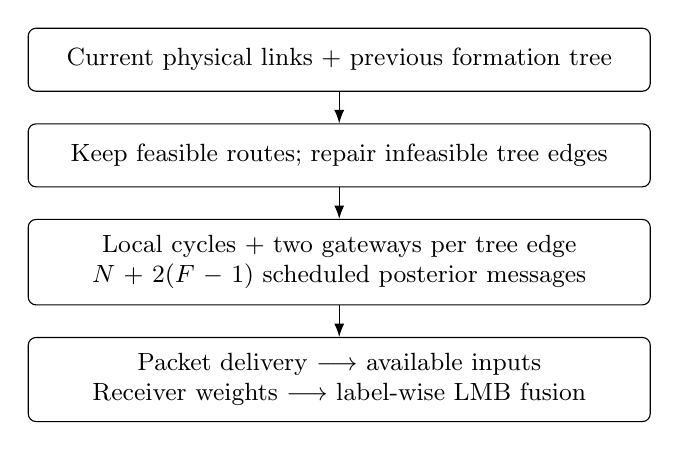
\begin{tikzpicture}[node distance=4mm, font=\small,
 box/.style={draw,rounded corners=1mm,align=center,text width=7.5cm,
 minimum height=8mm,inner sep=2mm}, >=Latex]
\node[box] (a) {Current physical links + previous formation tree};
\node[box,below=of a] (b) {Keep feasible routes; repair infeasible tree edges};
\node[box,below=of b] (c) {Local cycles + two gateways per tree edge\\
$N+2(F-1)$ scheduled posterior messages};
\node[box,below=of c] (d) {Packet delivery $\longrightarrow$ available inputs\\
Receiver weights $\longrightarrow$ label-wise LMB fusion};
\draw[->] (a)--(b);\draw[->] (b)--(c);\draw[->] (c)--(d);
\end{tikzpicture}
\caption{The routing and fusion pipeline. Scheduled connectivity is a
property of the third stage; actual information use also depends on delivery
and label availability in the fourth stage.}
\label{fig:method}
\end{figure}

\noindent\textbf{Proposition 1 (scheduled backbone).}
If every local cycle and every directed gateway is physically feasible,
the scheduled sensor graph is strongly connected and contains exactly
\begin{equation}M=N+2(F-1)\label{eq:messages}\end{equation}
directed messages per round.
\emph{Proof.} The local cycles contribute $N$ edges and provide directed
paths between sensors in each formation. The tree contributes $F-1$
formation edges, each realized in both directions. Concatenating local
paths and gateways gives a directed path between any two sensors.
The edge sets are disjoint, giving (\ref{eq:messages}).
This is a count for the chosen architecture, not a global lower bound over
all strongly connected directed graphs or a guarantee about delivered links.

\section{Packet Delivery and Finite-Round Fusion}
\subsection{Where a missing weight goes}
Let $W$ be a planned row-stochastic matrix with positive diagonal.
For receiver $i$, let $D_{ij}\in\{0,1\}$ indicate delivery, set $D_{ii}=1$,
and define missing weight mass $m_i=\sum_{j:D_{ij}=0}W_{ij}$.
The current reference implementation omits an unavailable input and uses
\begin{equation}
 R_{ij}=\frac{W_{ij}D_{ij}}{1-m_i}.\label{eq:renorm}
\end{equation}
This differs from the planned removal of a local edge. An existing
alternative receiver rule returns missing mass to self:
\begin{equation}
 S_{ij}=W_{ij}D_{ij}+m_i\mathbf1\{i=j\}.\label{eq:self}
\end{equation}
Both are row stochastic, and both satisfy
$\|R_{i:}-W_{i:}\|_1=\|S_{i:}-W_{i:}\|_1=2m_i$.
Their distinction is therefore not a smaller row-wise perturbation norm.
Rule (\ref{eq:self}) preserves the planned weight of each surviving
neighbor. If a 0.70-weight dominant input is missing, a surviving
0.05-weight input becomes $0.05/0.30=0.1667$ under
(\ref{eq:renorm}), but stays at 0.05 under (\ref{eq:self}).
The latter avoids amplification but can slow useful information transfer.

Neither rule preserves double stochasticity under arbitrary directed
losses. For example, a symmetric two-node matrix with off-diagonal weight
$a$ becomes $\left[\begin{smallmatrix}1&0\\a&1-a\end{smallmatrix}\right]$
after one direction fails under self fallback. Its column sums are
$1+a$ and $1-a$. Reciprocal scheduled gateways alone consequently do not
establish equal-weight KLA consensus after packet loss.

\subsection{A finite-round sensitivity bound}
The following bound concerns exact geometric fusion of \emph{fixed}
positive densities on a common support. It does not assume new observations
between consensus rounds. Write
\begin{equation}
 q_\alpha(z)=\frac{\prod_jq_j(z)^{\alpha_j}}
 {\int\prod_jq_j(u)^{\alpha_j}\,du},\qquad
 \alpha\geq0,\quad\mathbf1^\top\alpha=1.
\end{equation}
Assume the log-density oscillation on this support is bounded:
$\osc(\log q_j)=\sup_z\log q_j(z)-\inf_z\log q_j(z)\leq L$.
For any two coefficient vectors $\alpha,\beta$,
\begin{equation}
 D_{\rm KL}(q_\alpha\|q_\beta)\leq L\|\alpha-\beta\|_1.
 \label{eq:bound}
\end{equation}
To see this, put $h=\sum_j(\alpha_j-\beta_j)\log q_j$.
Its oscillation is at most $L\|\alpha-\beta\|_1$.
The log normalization ratio lies between $\inf h$ and $\sup h$,
so the log density ratio, and its expectation, are bounded above by
the same oscillation.

Let $P=\widetilde W_K\cdots\widetilde W_1$ and
$Q=W_K\cdots W_1$ be delivered and planned products. The induced
infinity norm is submultiplicative and equals one for each stochastic
factor. A telescoping expansion therefore gives
\begin{equation}
 \max_i\|P_{i:}-Q_{i:}\|_1
 \leq\sum_{k=1}^K\|\widetilde W_k-W_k\|_\infty
 \leq 2\sum_{k=1}^K\max_i m_{i,k}.\label{eq:product}
\end{equation}
Equations (\ref{eq:bound})--(\ref{eq:product}) connect lost weight mass
to deviation from the scheduled geometric pool. They do not favor one
fallback rule, imply lower ground-truth error, or establish uniform
averaging. Gaussian densities on unbounded support need not satisfy the
oscillation assumption. Mixture truncation, changing label support and
intervening Bayesian updates additionally prevent treating this bound as a
guarantee for the full implemented tracker.

\section{Experiments and Remaining Tradeoffs}
\subsection{Paired protocol}
We use a temporally coupled formation-braid simulation with four or six
formations of six sensors, denoted M24 and X36. The scenes contain 16 and
24 targets over 160 time steps. Sensors within a formation share a heading,
with a $120^\circ$ field of view and 300\,m sensing range. Detection
probability is 0.88, clutter rate is 4 and measurement noise standard
deviation is 7\,m. Target handovers overlap periods of physical route
failure. Each scale uses seed 1301; truth, measurements, directed delivery
uniforms and filter randomness are paired across its arms.

The fixed baseline keeps its initial formation-tree edges; infeasible
connections are dropped. Full causal repair retains two inputs per receiver
and changes the formation tree when required. Sparse causal repair uses
(\ref{eq:messages}). These three arms share packet renormalization
(\ref{eq:renorm}). A separate full-episode X36 run of (\ref{eq:self}) is
in progress and is not included as a completed result.

All arms use a componentwise powered-Gaussian-mixture approximation to KLA:
at most three input components, eight fused components and 256 component
tuples. This preserves multiple modes but is not an exact arbitrary-GM power.
Label-absence handling is held fixed across arms. The implementation uses
one communication/fusion round per tracking step.

We report position-only Euclidean OSPA (E-OSPA), with order 2 and cutoff
150\,m \cite{schuhmacher2008ospa}, and conditional Hungarian-matched position
RMSE. E-OSPA is averaged over sensor--time pairs; RMSE averages their finite
matched-set RMSE values, excluding a nonempty set paired with an empty set.
The latter must be interpreted alongside absolute cardinality error.
Focus consistency is mean pairwise E-OSPA between one fixed representative
per formation over $t=40$--140, not an all-node agreement measure.
Communication cost is attempted posterior-payload bytes, including failed
transmissions, but excluding routing-control traffic.

\begin{table*}[t]
\centering
\caption{Complete paired development episodes, seed 1301. Lower values are
better in all four metric columns. Error measures are in metres; bytes are
decimal MB of attempted posterior payload. Messages are scheduled, before
delivery. Each scale has its own fixed baseline; no confidence intervals
can be inferred from a single seed.}
\label{tab:main}
\small
\begin{tabular}{llrrrrr}
\toprule
Scale & Routing policy & E-OSPA & Cond. RMSE & Focus consistency & Payload & Messages/step\\
\midrule
M24 & Fixed formation tree &125.478&22.640&133.599&40.769&46--48\\
    & Full causal repair &\textbf{122.380}&14.081&131.913&44.867&48\\
    & Sparse causal repair &122.462&\textbf{12.183}&\textbf{131.664}&\textbf{36.676}&30\\
\midrule
X36 & Fixed formation tree &132.680&36.925&139.407&76.871&66--72\\
    & Full causal repair &\textbf{131.795}&19.586&\textbf{139.004}&81.259&72\\
    & Sparse causal repair &132.192&\textbf{19.329}&140.489&\textbf{60.090}&46\\
\bottomrule
\end{tabular}
\end{table*}

\subsection{What the comparisons establish}
Table~\ref{tab:main} separates repair from sparsification. Full causal
repair improves the three reported error measures over fixed routing at
both scales, but increases attempted bytes by 10.052\% on M24 and
5.708\% on X36. The sparse policy instead saves 10.041\% and 21.830\% of
attempted bytes. On M24 its E-OSPA and conditional RMSE improve by
2.403\% and 46.190\%, and focus consistency improves by 1.449\%.
However, the worst formation-wise RMSE change is a 24.085\% degradation.

On X36 sparse repair improves E-OSPA by only 0.368\% despite a
47.655\% conditional-RMSE reduction. Mean absolute cardinality error rises
from 18.456 to 18.597, and focus consistency worsens by 0.776\%.
Consequently, the RMSE decrease cannot be interpreted as a comparable
improvement in complete target-set recovery. The large cardinality errors
also show that the global target-set task remains difficult under limited
views and finite communication.

A packet-only replay using the same delivery uniforms finds that the
sparse graph is strongly connected after delivery on 41/160 M24 steps
and 18/160 X36 steps. Planned matrices are non-doubly-stochastic on
17 and 22 steps, whereas packet-renormalized matrices are non-double on
122 and 143 steps. This replay assumes that a delivered packet supplies an
input; empty payloads and label-specific censoring can further restrict
fusion. The counts do not prove absence of connectivity over longer
windows or identify the cause of the tracking differences.

\subsection{Limits and next discriminating experiment}
The next controlled comparison retains the sparse topology and changes
only the missing-input rule to (\ref{eq:self}). It asks whether avoiding
surviving-neighbor amplification improves E-OSPA, cardinality and consistency
while retaining the byte advantage. Its outcome is not assumed by the
analysis. A positive result must be checked on M24 before further tuning.
Frozen multi-seed tests and a separate non-radial zipper-merge scene are
then required to evaluate reproducibility and geometry dependence.

The current evidence does not establish statistical significance,
end-to-end control-inclusive bandwidth savings, or a decentralized routing
implementation. The message count and perturbation arguments are analytical
properties of the stated construction and assumptions; their usefulness for
set estimation must be demonstrated rather than inferred from connectivity.

\section{Conclusion}
Sparse causal routing provides a concrete communication advantage over a
fixed formation tree in two paired development cases. Its joint tracking
benefit remains incomplete: conditional localization gains coexist with
cardinality, consistency and formation-tail tradeoffs. The resulting research
direction is delivery-aware sparse fusion, with actual received inputs as
the link between topology design and finite-round LMB estimation.

\section*{Acknowledgements and declarations}
This work received no external funding. The authors declare no conflicts
of interest. The experiments use synthetic simulation data.
\bibliographystyle{IEEEbib}
\bibliography{references}
\end{document}
